\section{Learning to Play a Game through Self-Play}
\subsection{Overview of the problem}
The final problem is to learn to play a game through self-play using parallel agents.  The focus is on the ultimate quality of the agent produced, with less emphasis on the speed of learning.  In this problem the agent is pre-programmed with knowledge about how the game works.  That is the agent can determine the next state of the game for any of the actions that are possible from the current state.  It also can determine which actions are legal actions from the current state.  The agent does not know the goal of the game and can not determine in advance what board positions are wins or losses, which must be learned through the reward signal.  The game uses the knight piece from chess on a 5 x 7 chessboard.  The game’s piece movement pattern, number of pieces per side, and board size are variable problem parameters but the results shown here are for knights on a 5 x 7 board and the game starts with the random placement of 5 pieces for each player.  Each player makes a move, as in chess, and a player wins if all opponent’s pieces are captured.  The game has a maximum number of turns and the result is a drawn game when that limit it is reached.

Learning through self-play was advanced by the famous work by Tesauro (Tesauro, 1994) who used TD($\lambda$) and self play to train a program to play backgammon at a master level.  This was dramatic accomplishment and has not yet been duplicated in other domains.  Tesauro points out in his work that it may be the random element that is present in backgammon that drives the learning agent into wide exploration of the state space, enabling high quality learning to take place during self-play.  The random element helps to avoid the problem of converging prematurely to a sub-optimal strategy that can happen with deterministic games.  In those games, the agent may only experience a small fraction of the state space and optimizes for this region only, since by playing itself, it never has to deal with other regions of the state space.

This game is discrete but has a large state/action space.  There are ${35 \choose 5} \times {30 \choose 5}$ possible starting positions with random placement of 5 Xs and 5 Os on a 5 by 7 board.  The total number of game states is even larger since pieces can be removed during the game.  The five knights can move in up to 8 directions each so there may be up to 40 possible actions.  Clearly, there are too many values to learn either $V(s)$ or $Q(s,a)$ for every point and generalization is required.  For this problem I chose to use a neural net to approximate the value function $V(s)$.  The value function can be used by the agent to pick optimal moves with one move look ahead.  The agent loops through possible moves, calculates the board position after each one and selects the move that results in the highest value board position.

\subsection{Neural Net Design}
The neural net must take a description of the board position and output the agent’s estimated value for that board position, $V(s)$.  I coded the board position as two series of binary values for each square on the board.  The first series had the value 1 when player X had a piece on the corresponding square and the second series indicated squares with an O piece.  A single layer of 4 hidden nodes with sigmoid activation is used and the single output node uses sigmoid activation as well.  The number of hidden nodes is a parameter that can vary.  The neural net design is shown Figure ~\ref{fig:neural_net}.

\end{flushleft}
\begin{figure}[hbtp]
\center
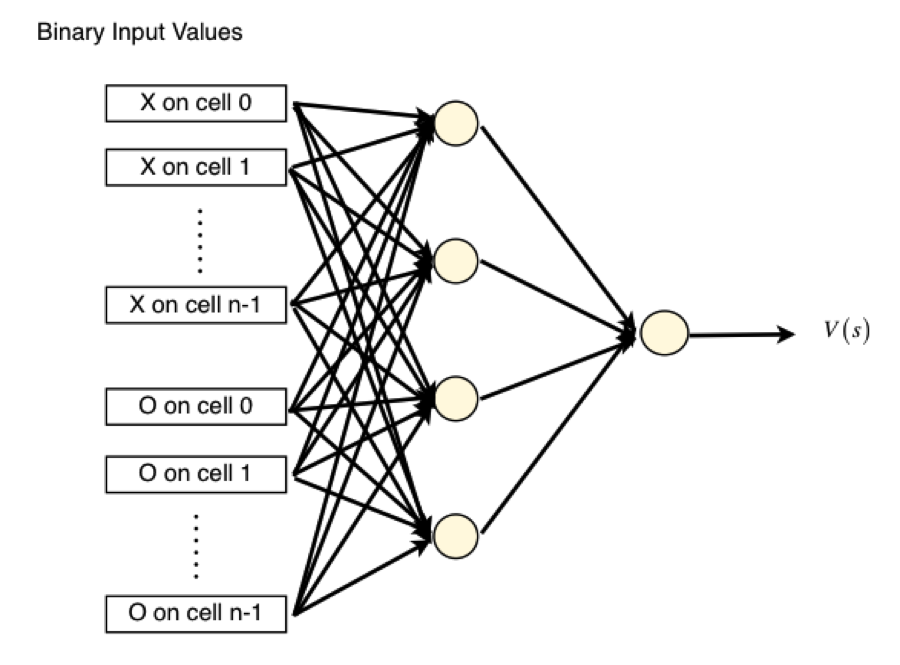
\includegraphics[scale=0.8]{fig11}
\caption{Neural net design for approximating $V(s)$}
\label{fig:neural_net}
\end{figure}
\begin{flushleft}

The learning algorithm for this problem is TD($\lambda$), building on the work done for the previous problems and adapting it to learn the $V(s)$ values.  The weight update rules combine the temporal difference equation for the value function with eligibility traces and back propagation updates for neural net weights.

The basic framework for learning is to have a group of agents learn by playing a set of games against each other.  The relative quality can be gauged by recording the agent’s winning percentage during the learning episodes.  This is shown for an 8-agent group in Figure 23.  The absolute measurement of agent quality requires some outside benchmark or test to be performed.  A benchmark opponent was used to gauge agent quality in Figure 24.  The quality measure is winning percentage calculated as $(wins + draws/2)/games$.

\end{flushleft}
\begin{figure}[hbtp]
\center
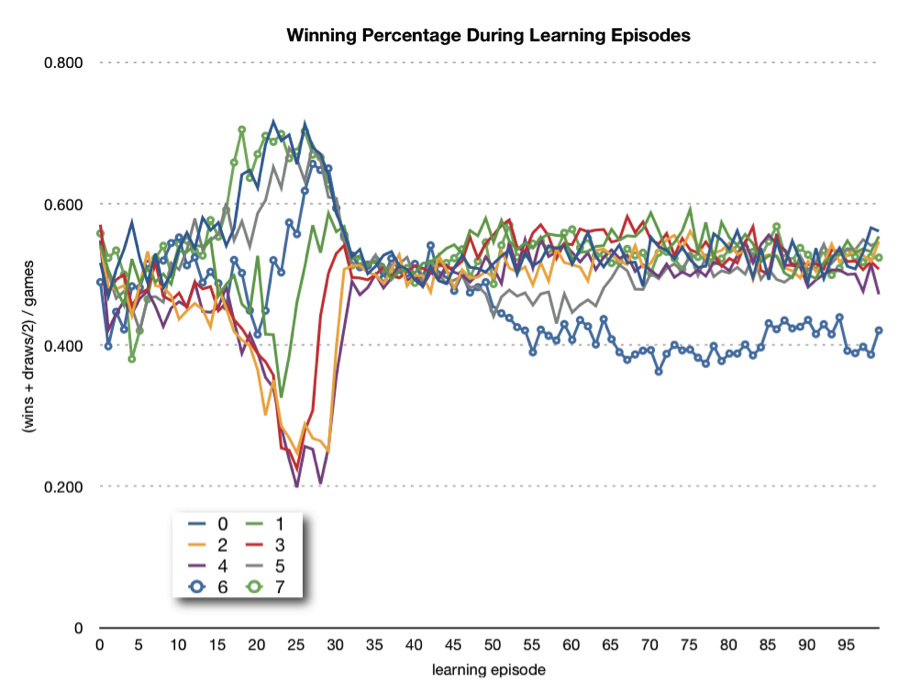
\includegraphics[scale=0.5]{fig12}
\caption{Learning through self-play winning percentage against other agents.}
\label{fig:sp_learning1}
\end{figure}

\begin{figure}[hbtp]
\center
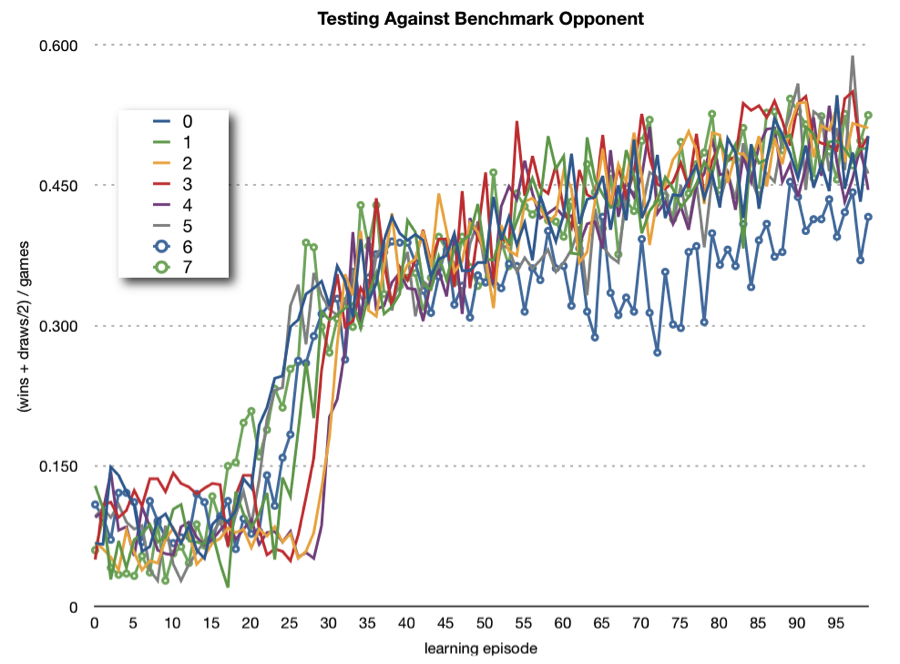
\includegraphics[scale=0.5]{fig13}
\caption{Learning through self-play winning percentage against fixed benchmark opponent.}
\label{fig:sp_learning2}
\end{figure}
\begin{flushleft}



 The GPU is much slower than the CPU for a single agent, but equals CPU speed with 4 agents and is faster for agent groups of 16 or more, as shown in Figure ~\ref{fig:time_per_million}, which displays the learning time for one million turns.

\end{flushleft}
\begin{figure}[hbtp]
\center
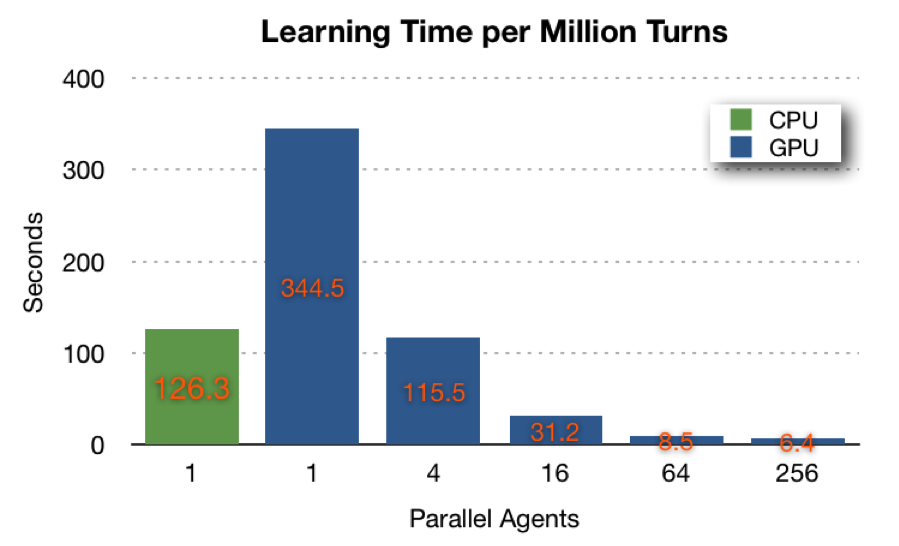
\includegraphics[scale=0.8]{fig17}
\caption{Speed of learning by agent group size.}
\label{fig:time_per_million}
\end{figure}

\begin{flushleft}

\subsection{Multiple Use of Parallelism}
The parallelism on the GPU was used for mulitple purposes on this problem.  For earlier problems one thread was assigned to each agent, allowing them to learn in parallel.  On this problem there we used multiple threads within each agent to speed up the expensive computations associated with neural net activation and updates.  In addition, we used parallelism to have each agent compete against multiple opponents simultaneously.  This approach requires creating multiple copies of the agent’s weights. Each copy then competes against a different opponent and updates its own weights. At the end of an episode of learning, the change in weights across all the copies of an agent is accumulated and the master copy is updated in one batch.  Using many threads within each agent and for simultaneous play by each agent resulted in the use of a smaller number of total agents.

\subsection{Replication with Variation and Summary of Results}
There is no direct sharing between parallel agents in this problem.  Indirect sharing happens by agents competing against each other and learning.  If one agent’s quality improves, it becomes a better opponent for the other agents and the other agents should improve as a result as well.

This problem produces a wide variation of agent quality, similar to Mountain Car problem.  Selecting the best agent from a group of parallel agents, based on internal competition between agents or testing against a benchmark opponent, will improve the quality compared to the average result.  Variation in quality can be seen in Figure ~\ref{fig:learn_v_benchmark}, which shows the best, worst, and average agent quality for a group of 64 parallel agents with quality measured against a benchmark opponent.

\end{flushleft}
\begin{figure}[hbtp]
\center
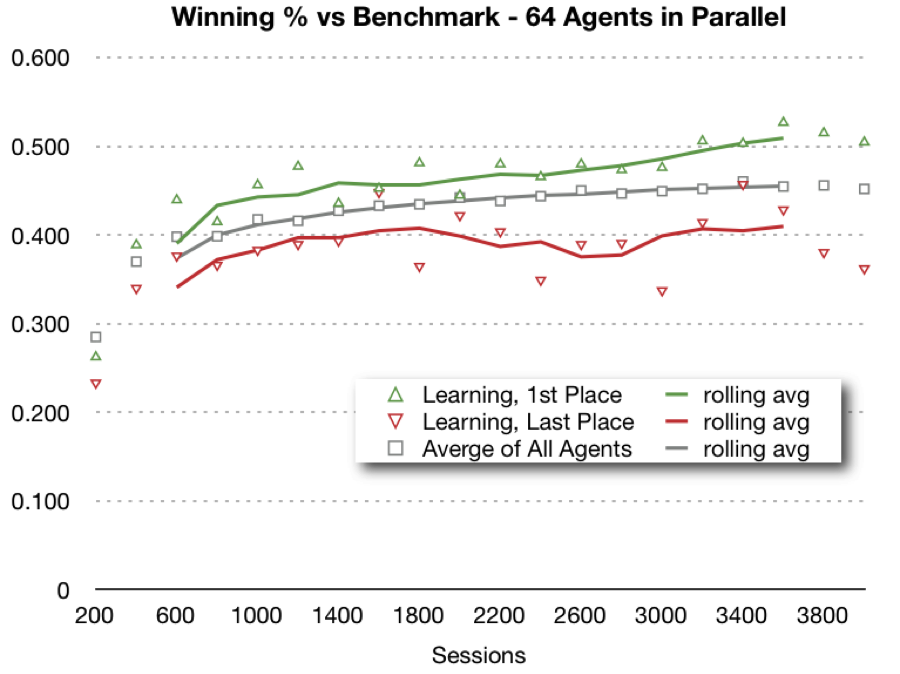
\includegraphics[scale=0.8]{fig18}
\caption{Learning through self-play against benchmark opponent}
\label{fig:learn_v_benchmark}
\end{figure}
\begin{flushleft}


Another technique that works on this problem is the use of selective replication to improve the overall quality of the agent population.  After each learning episode a round-robin competition determines the relative quality of the agents.  The best agents are copied and the worst agents dropped.  In addition, this has a secondary effect of improving the opponents for all agents in the future.  Figure ~\ref{fig:seq_diag_self_play} shows the high-level sequence diagram for CPU and GPU coordination.

\end{flushleft}
\begin{figure}[hbtp]
\center
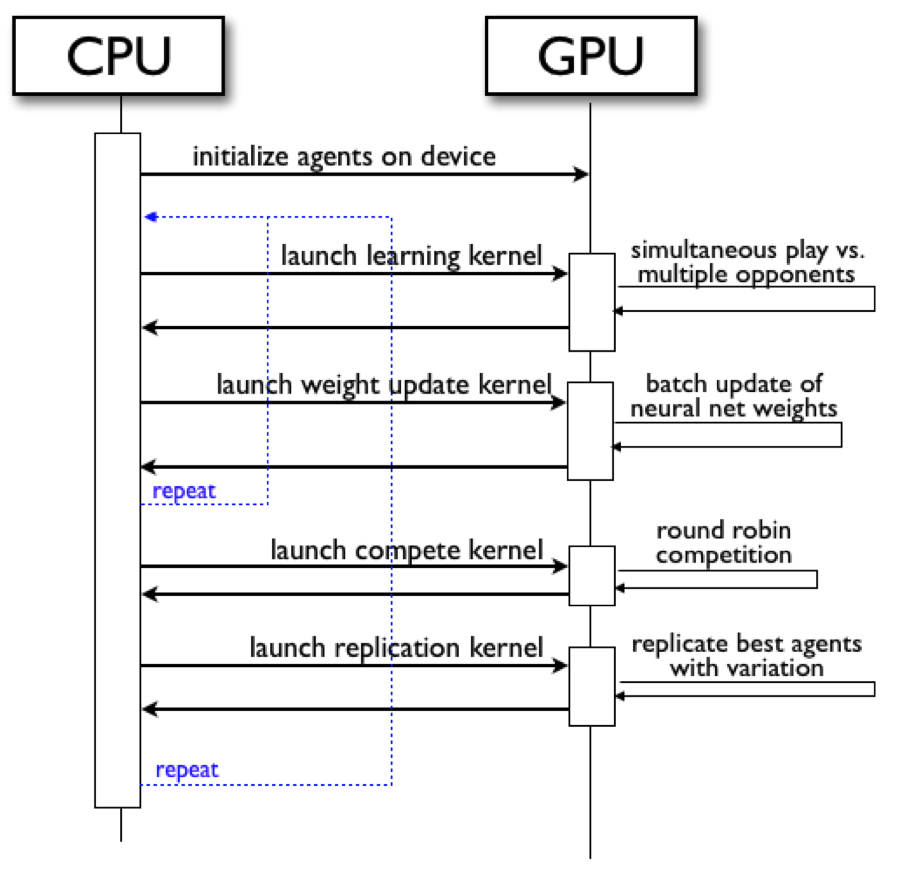
\includegraphics[scale=0.8]{fig19}
\caption{Sequence diagram for learning through self-play in parallel on GPU.}
\label{fig:seq_diag_self_play}
\end{figure}
\begin{flushleft}

The replicated copies of the best agents can include some differentiation.  They can have variation in the learning parameters or slight random bias applied to the neural net weights.  Variation helped the population of agents to continue to improve over a long training session.  The last graph, Figure ~\ref{fig:selection}, shows the typical results when using selective replication with variation with a group of 64 agents.  

\end{flushleft}
\begin{figure}[hbtp]
\center
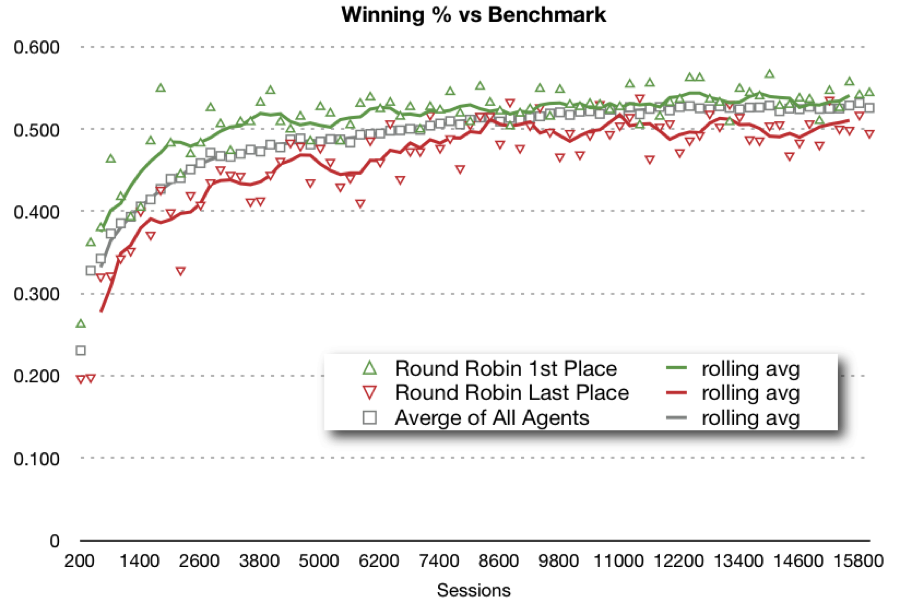
\includegraphics[scale=0.8]{fig20}
\caption{Learning through self-play with selective replication and variation.}
\label{fig:selection}
\end{figure}
\begin{flushleft}


The parallel approach to this problem provides a variety of opponents for agents to learn from.  This can help overcome the problems with self-play using a single agent.  In addition, the evolutionary techniques of selective replication with variation allow the population of agents to continue to improve over time.




